\begin{figure}
\begin{columns}
\begin{column}{0.05\textwidth}
\begin{subfigure}[b]{\textwidth}
\caption{}
\label{fig:natural}
\end{subfigure}
\end{column}
\begin{column}{0.27\textwidth}
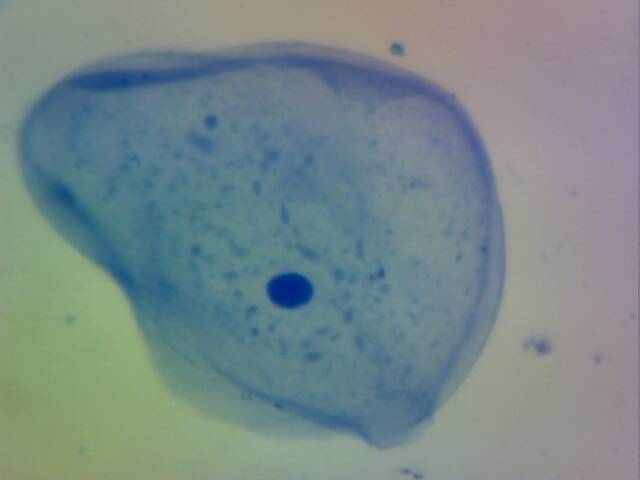
\includegraphics[width=\textwidth]{cheek_cell}
\end{column}
\begin{column}{0.07\textwidth}

\includegraphics[width=\textwidth]{arrow}
\end{column}
\begin{column}{0.27\textwidth}
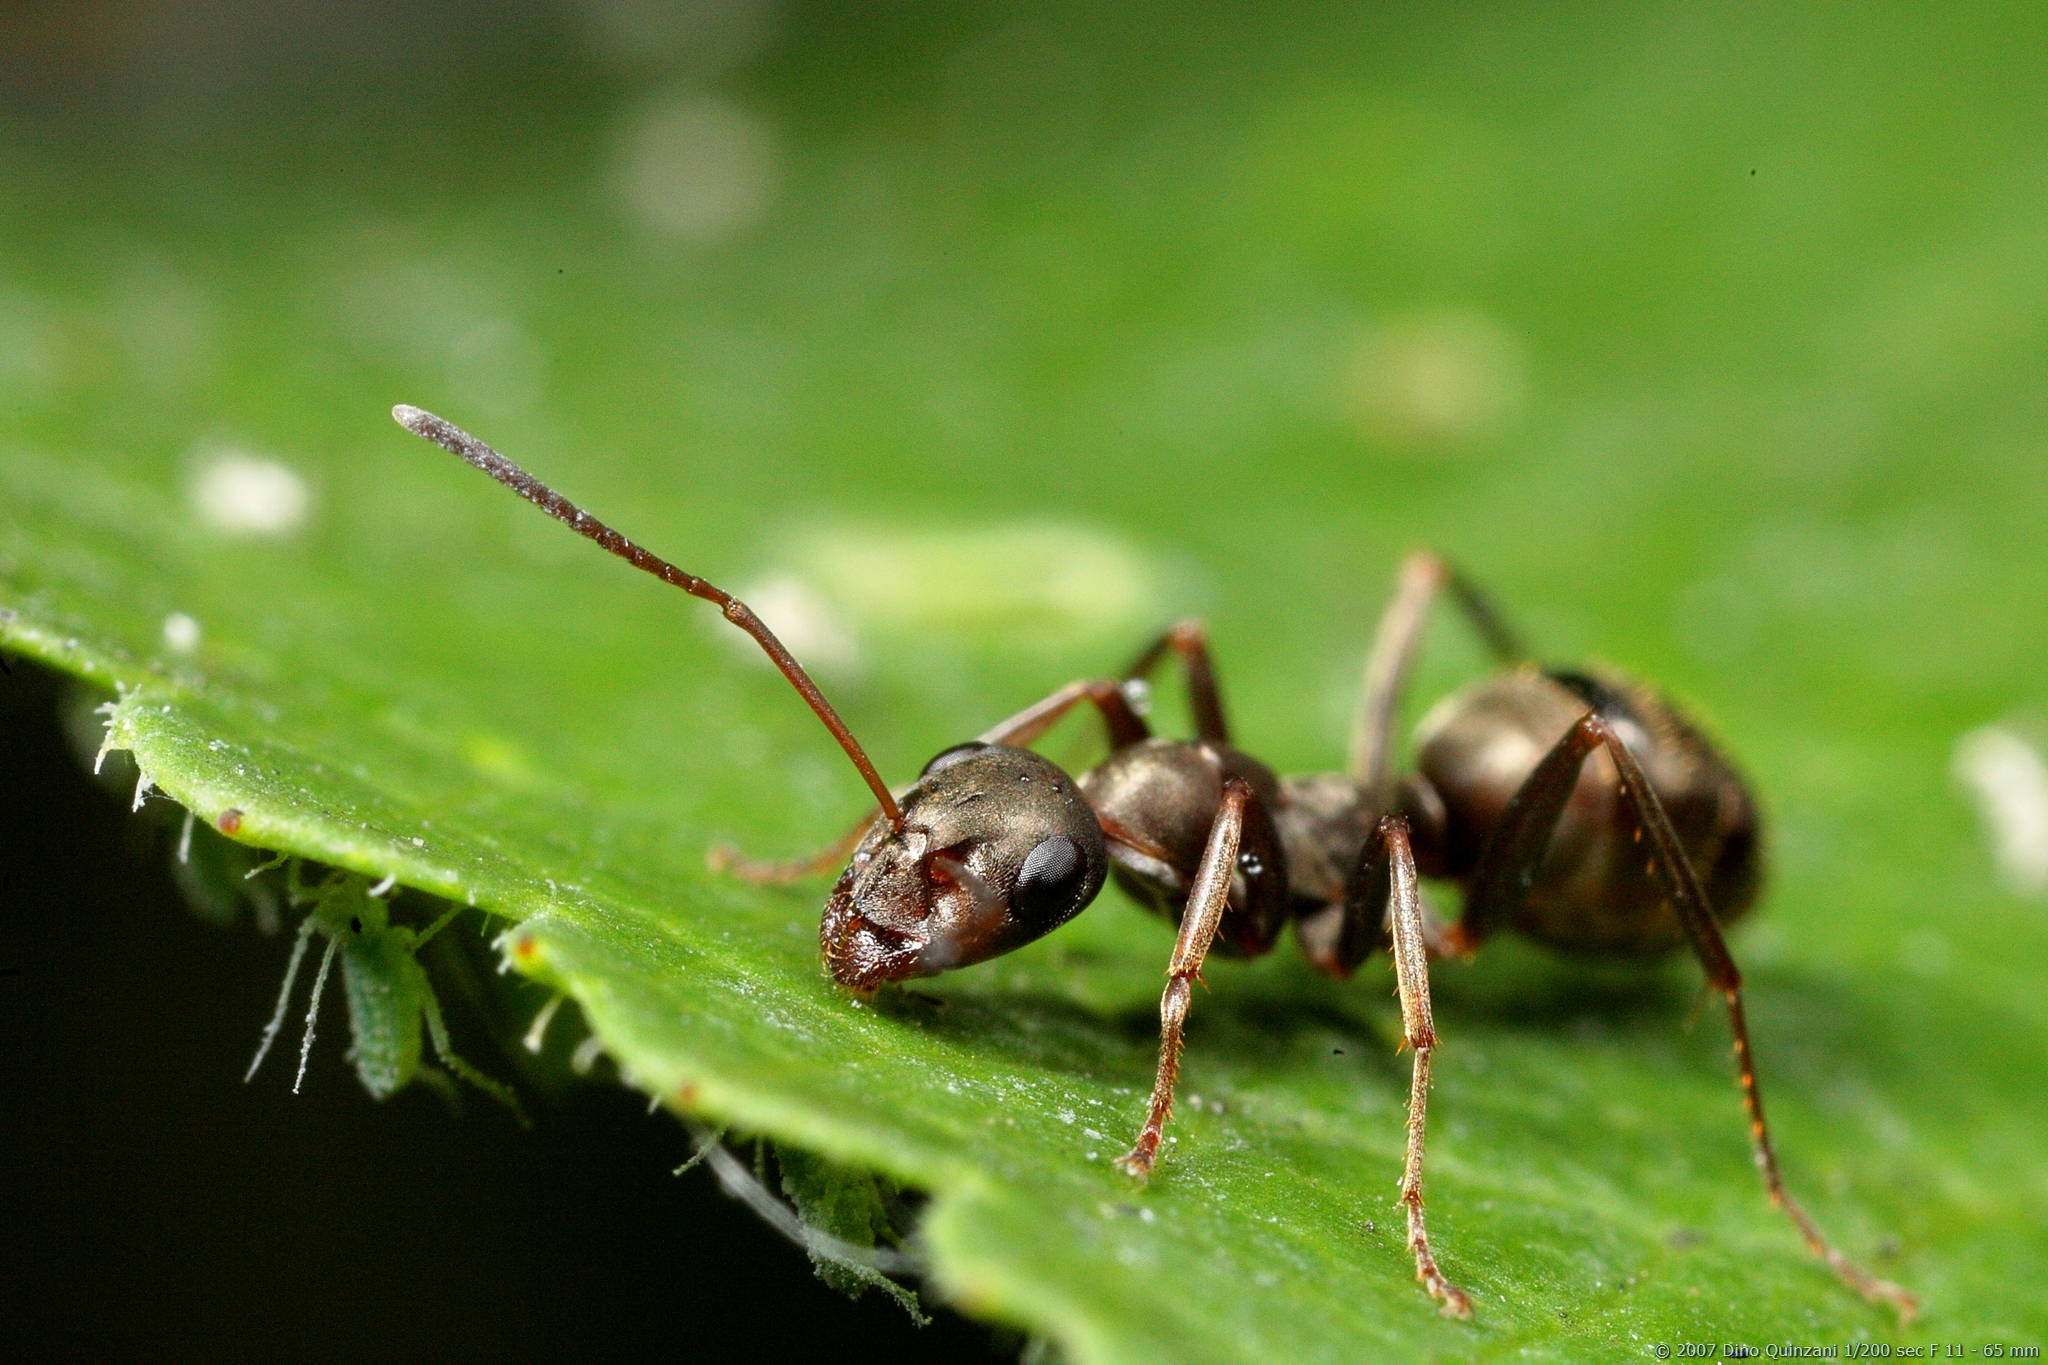
\includegraphics[width=\textwidth]{ant}
\end{column}
\end{columns}
\vspace{1ex}
\begin{columns}
\begin{column}{0.05\textwidth}
\end{column}
\begin{column}{0.27\textwidth}
\centering
cell {\tiny\cite{clare_and_ben_2017}}
\end{column}
\begin{column}{0.07\textwidth}
\end{column}
\begin{column}{0.27\textwidth}
\centering
ant {\tiny\cite{quinzani_2008}}
\end{column}
\end{columns}
\vspace{2ex}
\begin{columns}
\begin{column}{0.05\textwidth}
\begin{subfigure}[b]{\textwidth}
\caption{}
\label{fig:simulated}
\end{subfigure}
\end{column}
\begin{column}{0.27\textwidth}

\includegraphics[width=\textwidth]{cell}
\end{column}
\begin{column}{0.07\textwidth}
{\Large
\includegraphics[width=\textwidth]{arrow}}
\end{column}
\begin{column}{0.27\textwidth}
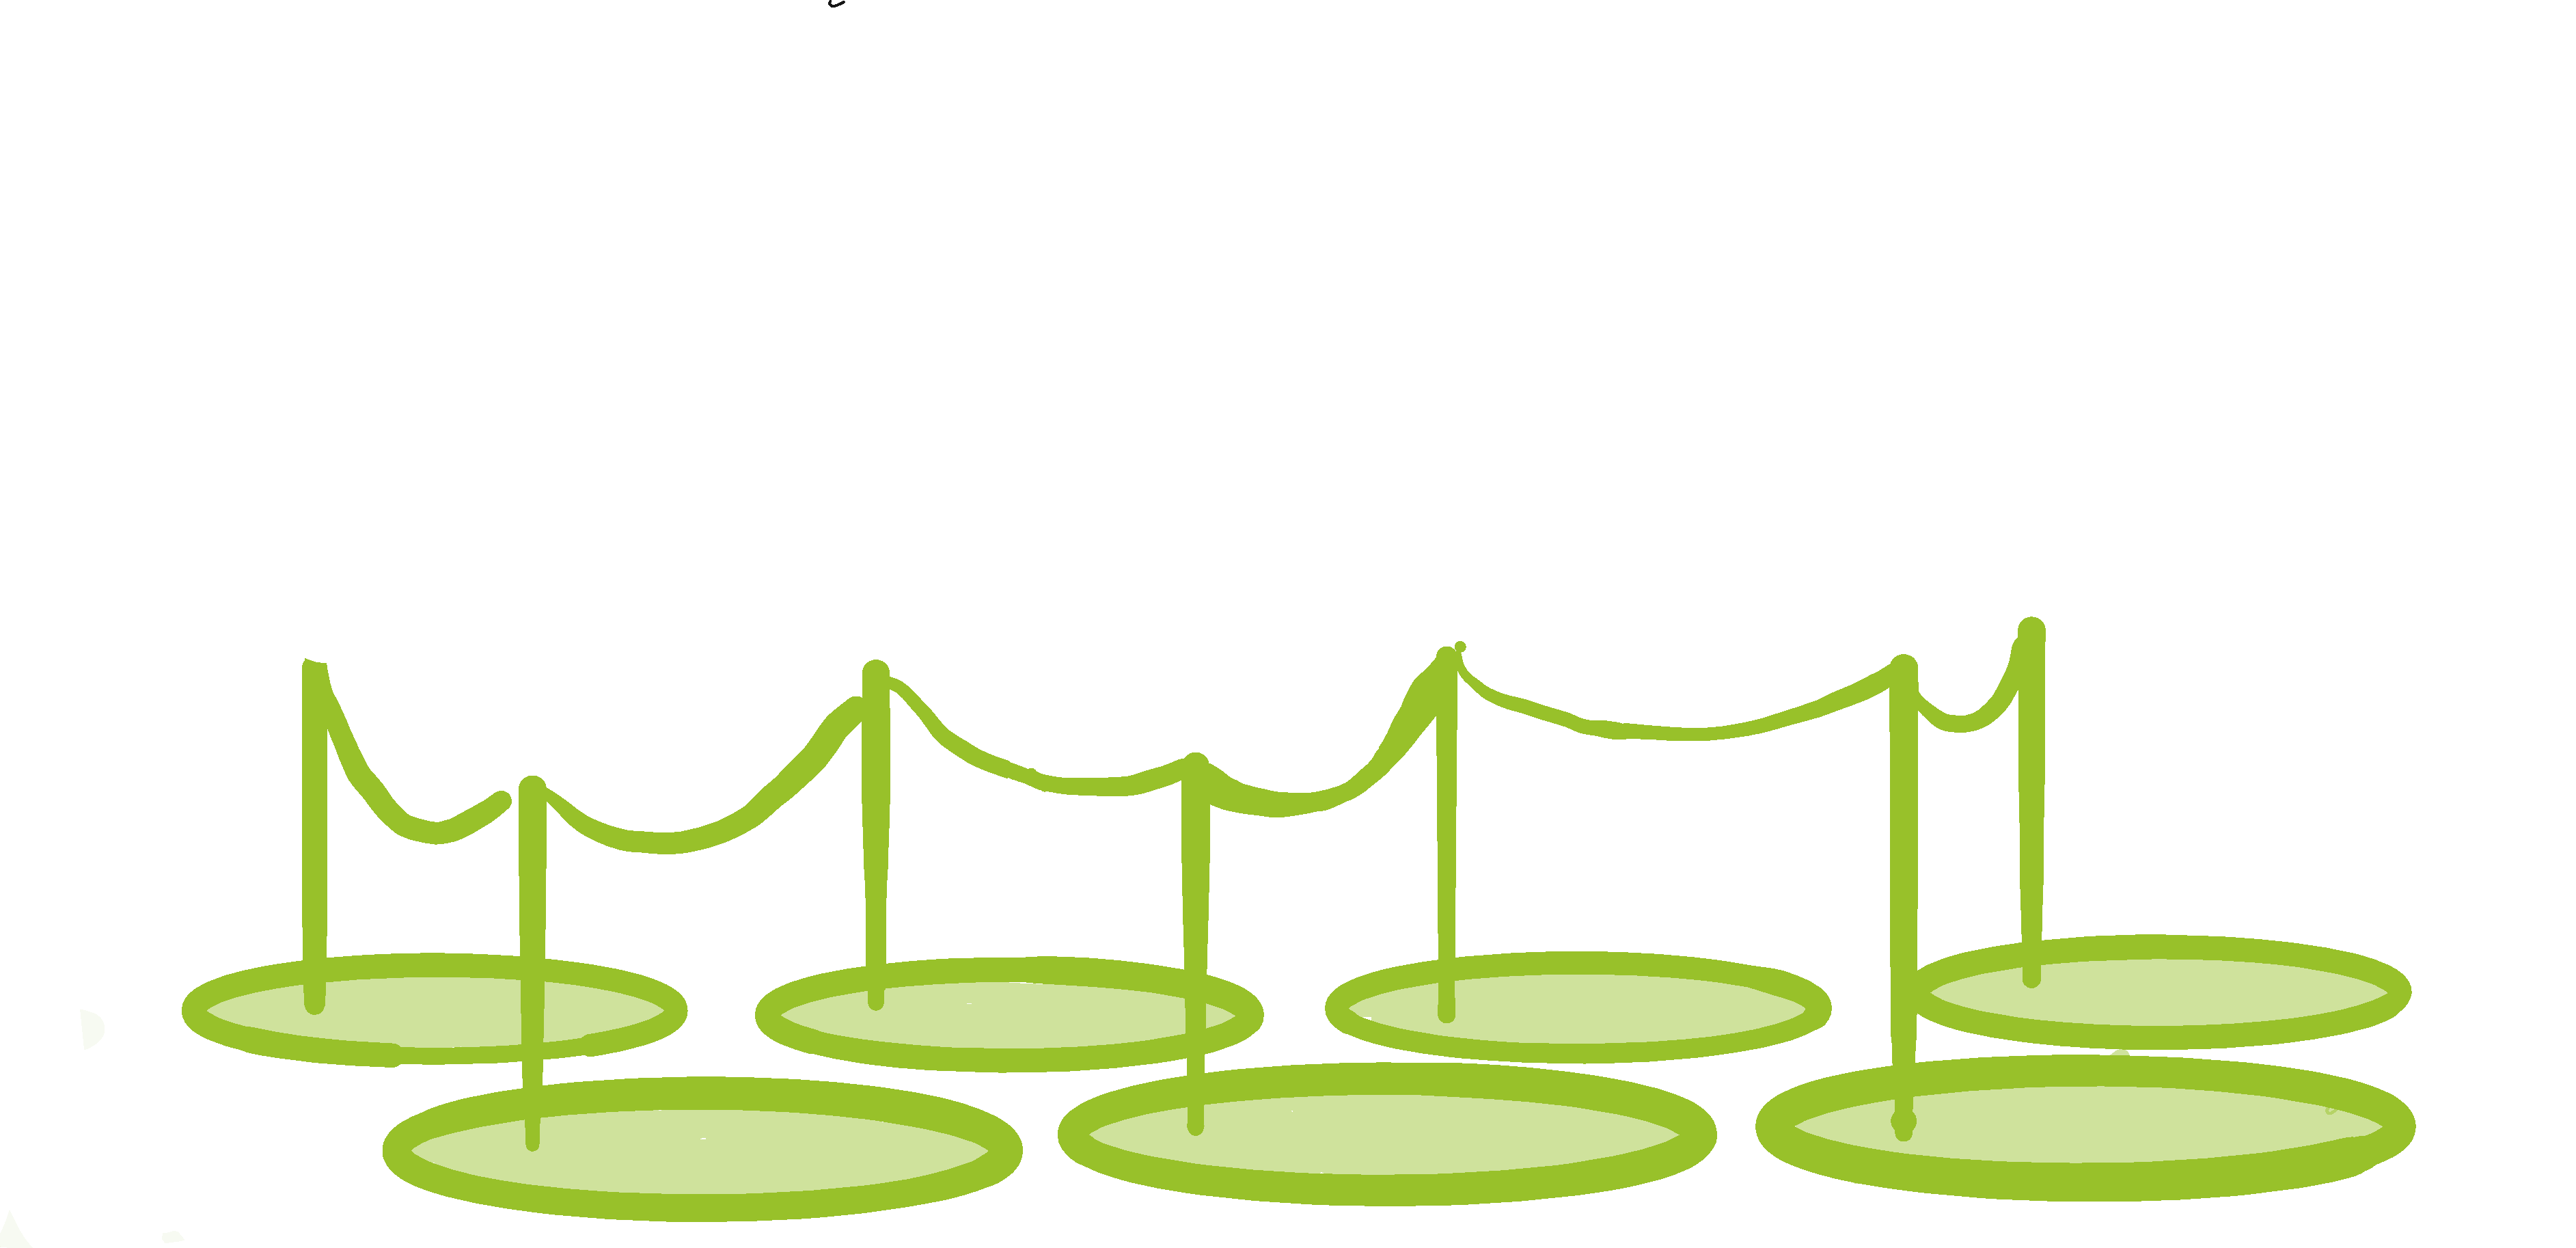
\includegraphics[width=\textwidth]{clump}
\end{column}
\end{columns}
\vspace{1ex}
\begin{columns}
\begin{column}{0.05\textwidth}
\end{column}
\begin{column}{0.27\textwidth}
\centering
cell
\end{column}
\begin{column}{0.07\textwidth}
\end{column}
\begin{column}{0.27\textwidth}
\centering
clump
\end{column}
\end{columns}
\vspace{2ex}
\caption{Analogy between (\subref{fig:natural}) natural and (\subref{fig:simulated}) simulated hierarchical fraternal transitions of individuality.}

\end{figure}
